\documentclass[11pt,letterpape, fleqn]{article}
\usepackage[lmargin=1in,rmargin=1in,tmargin=1in,bmargin=1in]{geometry}

% -------------------
% Packages
% -------------------
\usepackage{
	amsmath,			% Math Environments
	amssymb,			% Extended Symbols
	enumerate,		% Enumerate Environments
	graphicx,			% Include Images    
	lastpage,			% Reference Lastpage
	multicol,			% Use Multi-columns
	multirow,			% Use Multi-rows
	siunitx
}

\graphicspath{{./images/}}

\usepackage{wrapfig}

% -------------------
% Font
% -------------------
\usepackage[T1]{fontenc}
\usepackage{charter}    


% -------------------
% Heading Commands
% -------------------
\newcommand{\class}{Mu Alpha Theta}
\newcommand{\term}{2022-2023}
\newcommand{\head}[4]{%
\thispagestyle{empty}
\vspace*{-0.5in}
\noindent\begin{tabular*}{\textwidth}{l @{\extracolsep{\fill}} r @{\extracolsep{6pt}} l}
	\textbf{#1} & \textbf{Name:} & \makebox[5.75cm]{\hrulefill} \\
	\textbf{#2} & & \\
	\textbf{\class:\; \term} & & \\
\end{tabular*} \\
\rule[2ex]{\textwidth}{2pt} %
}


% -------------------
% Commands
% -------------------
\newcommand{\prob}{\noindent\textbf{Problem. }}
\newcounter{problem}
\newcommand{\problem}{
	\stepcounter{problem}%
	\noindent \textbf{Problem \theproblem. }%
}
\newcommand{\pointproblem}[1]{
	\stepcounter{problem}%
	\noindent \textbf{Problem \theproblem.} (#1 points)\,%
}
\newcommand{\pspace}{\par\vspace{\baselineskip}}
\newcommand{\ds}{\displaystyle}


% -------------------
% Header & Footer
% -------------------
\usepackage{fancyhdr}

\fancypagestyle{pages}{
	%Headers
	\fancyhead[L]{}
	\fancyhead[C]{}
	\fancyhead[R]{}
\renewcommand{\headrulewidth}{0pt}
	%Footers
	\fancyfoot[L]{}
	\fancyfoot[C]{}
	\fancyfoot[R]{}
\renewcommand{\footrulewidth}{0.0pt}
}
\headheight=0pt
\footskip=14pt

\pagestyle{pages}


% -------------------
% Content
% -------------------

\begin{document}
\head{Worksheet \#4}{Date:}
\centering

% Question 1: https://www.youtube.com/watch?v=aO7PAupqI7Y&list=PLDZcGqoKA84E2a0L6IS68hswD4iiUN2Cv&index=196
\begin{minipage}{\textwidth}
	\problem
    \noindent  
	\vspace{0.5cm}

	Calculate the minimum of $f(x) = \sqrt{(x-4)^2+(y-10)^2} + \sqrt{(x-44)^2+(y-19)^2}$. 
	
	Hint: it involves triangles and not circles.
	\vspace{9.5cm}
\end{minipage}

% Question 2: https://www.youtube.com/watch?v=Rjo-PcrKrB0&list=PLDZcGqoKA84E2a0L6IS68hswD4iiUN2Cv
\begin{minipage}{\textwidth}
    \problem
    \noindent 
    \vspace{0.5cm}

	Determine the value of $\angle APC$.

	\vspace{1cm}

    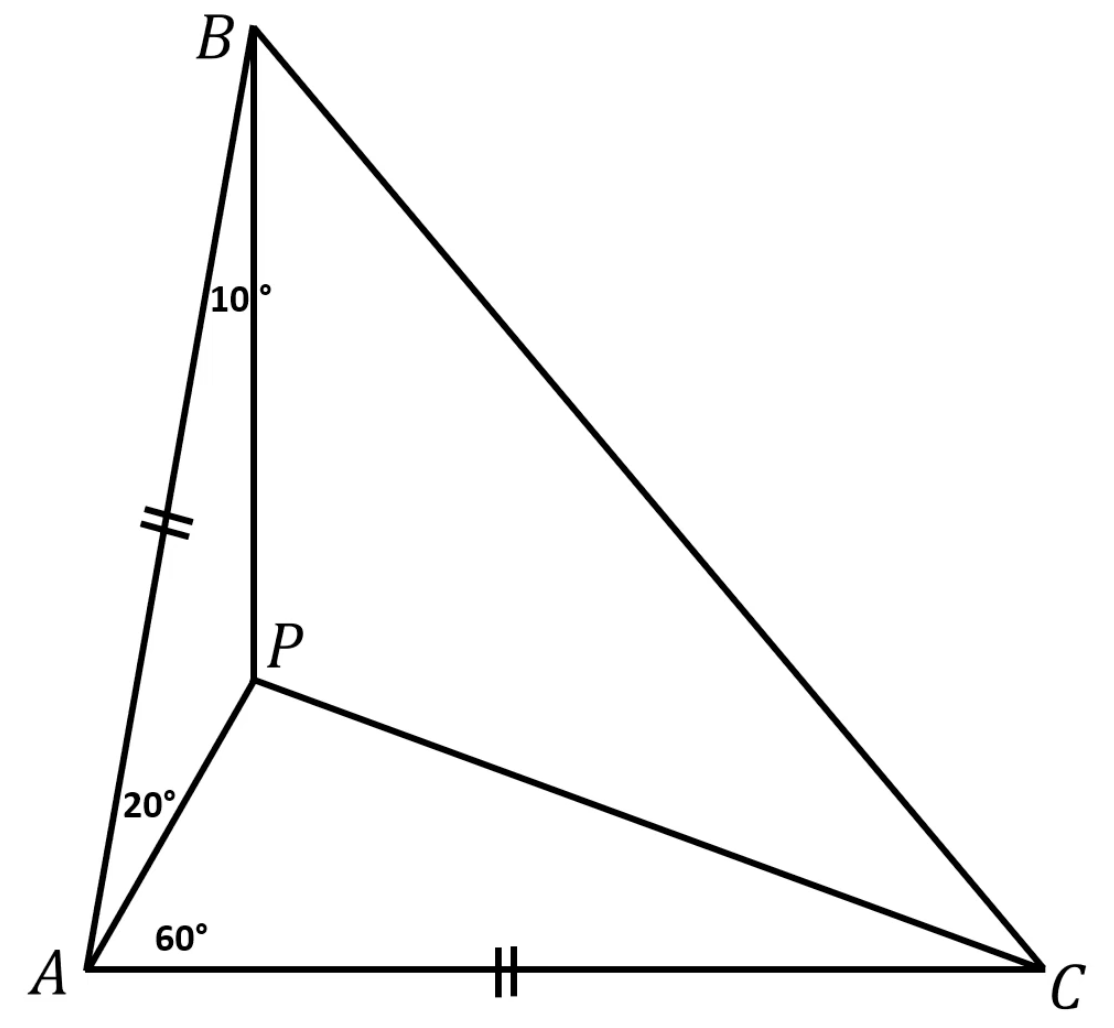
\includegraphics[width = 8cm]{images/q1.png}
\end{minipage}

\vspace{6cm}
\end{document}
